\documentclass[border=0.2cm]{standalone}
 
\usepackage{tikz}
\usetikzlibrary{trees}
 
\begin{document}
 
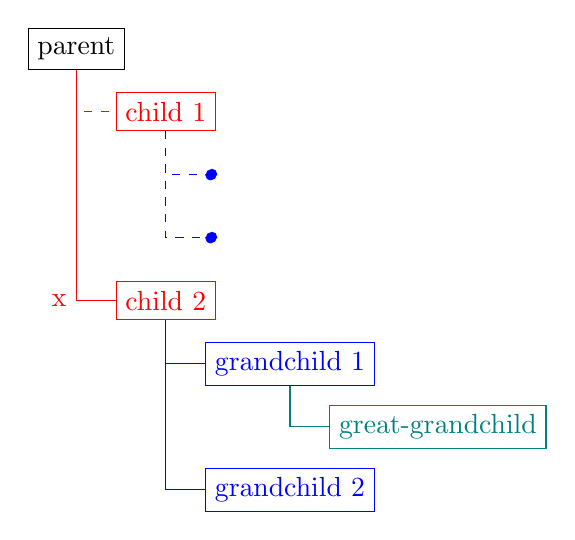
\begin{tikzpicture}
[
    level 1/.style = {red},
    level 2/.style = {blue},
    level 3/.style = {teal},
    every node/.append style = {draw, anchor = west},
    grow via three points={one child at (0.5,-0.8) and two children at (0.5,-0.8) and (0.5,-1.6)},
    edge from parent path={(\tikzparentnode\tikzparentanchor) |- (\tikzchildnode\tikzchildanchor)}]
 
\node {parent}
    child {node {child 1}
    child {node [circle, fill, minimum size = 4pt, inner sep = 0] {}}
    child {node [circle, fill, minimum size = 4pt, inner sep = 0] {}}
    edge from parent [dashed]} 
    child [missing] {}
    child [missing] {}
    child {node {child 2}
    child {node {grandchild 1}
    child {node {great-grandchild}}}
    child [missing] {}
    child {node {grandchild 2}}
    edge from parent node [draw = none, left] {x}};
 
\end{tikzpicture}
 
\end{document}